\documentclass[letterpaper]{article}
\usepackage{natbib,alifexi}
\usepackage{longtable}

\title{Analysis of the paper ``Ensemble Algorithms in Reinforcement Learning''}
\author{Jan van den Schilden$^{1}$, Nil Fernandez Lojo$^{1}$, Borel Kamdem$^{1}$ \and Siddheswar Mukherjee$^2$ \\
\mbox{}\\
$^1$Université Libre de Bruxelles, Belgium\\
$^2$Vrije Universiteit Brussel, Belgium }

\begin{document}
\maketitle

\begin{abstract}
This article presents the work of Wiering and van Hasselt in ``Ensemble
Algorithms in Reinforcement Learning'' \cite{wiering2008}. Ensemble methods
merge multiple reinforcement learning (RL) algorithms into a single
agent with the objectif of increasing the learning speed and the
obtained reward. While ensemble methods have already been used in the
context of reinforcement learning for representing and learning a single
value function \cite{singh1992, tham1995, sun1999}, Wiering and van Hasselt
introduce a novel technique that combines the policy of each RL
learning. The individual RL algorithms implemented were: Q-learning,
Sarsa, Actor-Critic, QV-learning, and ACLA. The ensemble methods are
majority voting, rank voting, Boltzmann multiplication, and Boltzmann
addition. They implemented their algorithms for 5 mazes problems with
increasing complexity to assess their performance. For all the mazes
except the first one, the state space is very large, therefore a neural
network was used for value functions approximation. We reimplemented
their algorithms and obtained the same results for the first maze. For
the other mazes, our neural network did not converge. Possible causes
for this non-convergence are discussed in this article.
\end{abstract}

\section{Introduction}\label{introduction}

Reinforcement learning is a branch of machine learning in which software
agents learn from interacting with their environment. It is a very
general framework that can be used to learn tasks of a sequential
decision making nature. An environment can exists as different states,
and the actions available to the agent depend on the state of this
environment. After every action, the agent receives a reward which might
be positive or negative. Through iterative experience, the agent seeks a
policy, an idea about which action needs to be performed for every
possible state of the environment, that maximizes the sum of rewards
over time.

For simple tasks, the agent can use a tabular expression to remember
values associated with certain states or state-action combinations, also
called state(-action) functions. For complex games however, there is an
explosion of state-action possibilities. Chess for example, is estimated
to have more than \(10^{50}\) chess-board configurations. Not only do we
lack the memory to store such a table, we would need more time than the
age of the universe to explore all possible states. Therefore function
approximators are used to approximate such state(-action) functions. The
capture the most essential concepts in order to maximize reward. Neural
networks are an example of such function approximator. DeepMind's
program AlphaZero is an interesting example that combines neural
networks with reinforcement learning algorithms to learn chess. The
program was given no domain knowledge except the rules and achieved a
superhuman level within 24 hours.

Some basic, well known online model-free value-function based
reinforcement algorithms are SARSA and Q-learning. They are both
temporal difference (TD) reinforcement learning algorithm that learn by
updating a Q-function (action value function). The difference is that
Q-learning is off-policy. This means that the optimal action-value
function is learned independent of the policy that is being followed,
unlike on-policy methods like SARSA, the learning of the action-value
does depend on the policy. The Actor-Critic (AC) is an temporal
difference, on-policy learning algorithm. But where SARSA and Q-learning
only keep track of a single Q-function, AC makes the distinction between
a critic value function V that only depends on the state, and an Actor
function which will map for each action the states to preference values.
\cite{wiering2007} explains a more recent and advanced on-policy QV-learning
method. This algorithm can be seen as mix between Actor-Critic and
Q-learning. As Actor-Critc, it learn the state-value function V and an
action-value function. But unlike Actor-Critic, it learns the Q-function
for that. ACLA is another on-policy RL algorithm derived from
Actor-Critic that learns a state value-function V and Actor function P.
QV-learning and ACLA have been shown to outperform similar, more basic,
RL algorithms \cite{wiering2007} and QV-learning even scores higher in
certain problem contexts than more recent RL methods \cite{wiering2009}.

Reinforcement learning methods, however useful, can take many steps to
learn. Ensemble methods are a powerful method to combine different
Reinforcement Learning (RL) algorithms, which often result in improved
learning speed and final performance. {[}1{]} used ensemble methods to
combine multiple reinforcement learning algorithms for multiple agents
for which they used Temporal-Difference(TD) and Residual-Gradient(RG)
update methods as well as a policy function. Other ensemble methods have
been used in reinforcement learning to combine value functions stored by
function approximators (\cite{wiering2008} {[}14{]}, {[}15{]}, {[}16{]},
{[}17{]}). However, only Rl algorithms with the same value function can
be combined in this way. \cite{wiering2008} wanted to combine RL methods with
different value functions and policies (e.g.~Q-learning and ACLA). It is
possible however, to combine the different policies that were derived
from distinct value functions. Some algorithms that perform this task
and take exploration into account at the same time are Majority voting,
Rank voting, Boltzmann multiplication, and Boltzmann addition. Majority
Voting (VM) combines the best action of the RL algorithms and bases the
final decision on the number of times that each action was preferred by
the different RL methods. Rank Voting (RV) lets each algorithm rank the
different actions and combines these rankings into final preferences over
actions. Boltzmann mulplication(BM) multiplies the Boltzmann
probabilities of each action computed by each RL algorithm. Finally,
Boltzmann Addition(BA) is very similar to Boltzmann mulplication, but
adds instead of multiplies the Boltzmann probabilities of actions.

In this article, we presents the work of Wiering and van Hasselt in
``Ensemble Algorithms in Reinforcement Learning''. Five RL algorithms
(Q-learning, SARSA, Actor-Critic, QV-learning, and ACLA) were compared
to 4 ensemble methods (Majority Voting, Rank Voting, Boltzmann
multiplication, and Boltzmann Addition). To this end, they had to solve
five mazes of varying complexity.

\section{Methods}\label{methods}

\subsection{Reinforcement learning}\label{reinforcement-learning}

With reinforcement learning methods, agent are able to learn from
interactions with their environment. We assume a Markov Decision Process
that is defined by the following parameters. The state-space \$ S
=\{s\_1, s\_2, \ldots{} , s\_n\}\$ with \(s_t\) denoting the state at
moment t. \(A(s)\) is the set of action that are available to the agent
if it is in state s, \(a_t\) is the action executes in state \(s_t\) at
time t. The transition function \(T(s,a,s')\) maps state-action pairs to
a probability over successor states. Finally, there is also the reward
function \(R(s,a,s')\) that return a reward for every state-action-state
transition. This reward function can give stochastic rewards. The goal
of an agent is to estimate the optimal policy \(\pi^*(s)\). With
\(\pi^*(s)\), the agent would know for each state what the optimal
action is to receive the highest possible cumulative discounted reward
in future states.

\subsubsection{Q-learning}\label{q-learning}

Q-learning is an off-policy, temporal difference (TD) reinforcement
learning algorithm that learns by updating a Q-function. This
action-value function Q directly approximates the optimal action-value
function \(Q^*\) and it does this independent of the policy that is
being followed. Q-learning updates with new experience
\((s_t, a_t, r_t, s_{t+1})\) in the following way:

\[Q(s_t,a_T) := Q(s_t,a_t) + \alpha ( r_t + \gamma max_a Q(s_{t+1}, a) - Q(s_t,a_t) )\]

With \(0 \leq \alpha \leq 1\) being the learning rate, and
\(0 \leq \gamma \leq 1\) being the discount factor. Higher \(\gamma\)
values will result in the agent taking into account not only the
immediate reward of an action, but also future rewards that will be
available in future states as a consequence of this action. The
advantage of tabular Q-learning is that it will always converge to
\(Q^*\). It does not matter what behavioral policy is used, as long as
each state-action pair is visited an infinite number of times (\cite{wiering2007} {[}13{]}). However, Q-learning combined with function
approximators, such as neural networks, have been observed to diverge
\cite{wiering2007}.

\subsubsection{SARSA}\label{sarsa}

Like Q-learning, SARSA is temporal difference (TD) reinforcement
learning algorithm that learns the action-value Q-function \cite{wiering2007}. Unlike Q-learning, SARSA is on-policy, meaning that the
approximation of optimal \(Q^*\) values depend on the policy being
followed (\cite{wiering2008} {[}6{]}). An experience is defined as the
quintuple \((s_t, a_t, r_t, s_{t+1}, a_{t+1})\). This quintuple is what
gave rise to the name SARSA (sutton 2018). After every transition,
Q-values are updated by the following method:

\[Q(s_t,a_T) := Q(s_t,a_t) + \alpha ( r_t + \gamma Q(s_{t+1}, a_{t+1}) - Q(s_t,a_t) )\]

As with tabular Q-learning, tabular SARSA converges towards \(Q^*\) if
all state-action pairs are visited an infinite number of times.

\subsubsection{Actor-Critic}\label{actor-critic}

The Actor-Critic (AC) is an temporal difference, on-policy learning
algorithm. Where SARSA and Q-learning only keep track on the Q-function,
Actor-Critic will update both a Critic and Actor function \cite{wiering2008}
{[}1{]}). The Critic function assigns values to the states, irrespective
of the action chosen by the agent. The Actor function will for each
action map the states to preference values \cite{wiering2008}. An experience
is defined as the sequence (\((s_t, a_t, r_t, s_{t+1})\)). After each
experience, the Critic and Actor get updated as follows {[}\cite{wiering2008}{[}11{]}{]}:

$$ \textrm{Critic: } V(s_t) := V(s_t) + \beta ( r_t + \gamma V(s_{t+1}) - V(s_t) ) $$

$$ \textrm{Actor: } P(s_t, a_t) := P(s_t, a_t) + \alpha ( r_t + \gamma V(s_{t+1}) - V(s_t) ) $$

Where \(\beta\) is the learning rate of the Critic and \(\alpha\) the
learning rate of the Actor. P-values should not be seen as literal
Q-values, but instead as preference values.

\subsubsection{QV-learning}\label{qv-learning}

QV-learning (\cite{wiering2008}{[}6{]}) is very similar to Actor-Critic. It is
also a learning method that learns a state value-function V with TD
method, and an Actor function to map the states for each action to
preference values. However, QV-learning learns actual Q-values as
preference values \cite{wiering2008}. After each experience
\((s_t, a_t, r_t, s_{t+1})\), the V value-function is updates in the
same way as in the Actor-Critic method \cite{wiering2007}:

\[ V(s_t) := V(s_t) + \beta ( r_t + \gamma V(s_{t+1}) - V(s_t) )   \]

The update for the Q-function is similar to the Actor update, but the
\(- V(s_t)\) at the end is replaced by \(- Q(s_t, a_t)\):

\[ \textrm{Qvalue: } Q(s_t, a_t) := Q(s_t, a_t) + \alpha ( r_t + \gamma V(s_{t+1}) - Q(s_t, a_t))\]

\subsubsection{ACLA (Actor-Critic Learning
Automaton)}\label{acla-actor-critic-learning-automaton}

Actor-Critic Learning Automaton (ACLA)(\cite{wiering2008}{[}6{]}) is an
on-policy learning algorithm that learns a state value-function V and
Actor function P. After each experience

\cite{wiering2008}\((s_t, a_t, r_t, s_{t+1})\), the state value-function is
updated in the same way as Actor-Critic or QV-learning \cite{wiering2007}:

\[ \delta_t = r_t + \gamma V(s_{t+1}) - V(s_t) \]

\[ V(s_t) := V(s_t) + \beta ( \delta_t ) \]

The actor function maps states to preferences for actions and is updated
by an automaton-like updating rule (\cite{wiering2008} {[}20{]}) The policy
mapping update depends on the sign of \(\delta\):

\(\delta_t \geq 0\)

\[ a = a_t: P(s_t, a_t) := P(s_t, a_t) + \alpha ( 1 - P(s_t, a_t)) \]

\[ \forall a \neq a_t:  P(s_T, a) := P(s_t, a) + \alpha ( 0 - P(s_t, a))\]

\(\delta_t < 0\)

\[ a = a_t: P(s_t, a_t) := P(s_t, a_t) + \alpha ( 0 - P(s_t, a_t)) \]

\[ \forall a \neq a_t:  P(s_t, a) := P(s_t, a) + \alpha \left( \frac{P(s_t, a)}{\sum_{b \neq a_t}P(s_t, b)} - P(s_t, a) \right)\]

There are also additional rules to ensure that the target values are
between 0 and 1 and existing. If \(P(s_t,a)\) is greater than 1, the
value gets changed to 1. If \(P(s_t,a)\) is smaller than 0, the value
gets changed to zero. If the denominator is 0, the new value equals
\(\frac{1}{|A| -1}\), with \(|A|\) being the number of actions \cite{wiering2008}.

\subsection{Ensemble algorithms in RL}\label{ensemble-algorithms-in-rl} 

Combining single classifiers for which the errors are not strongly
correlated can lead to a higher accuracy than what is available for a
single classifier. With this in mind, ensemble methods have been used in
reinforcement learning to combine value functions stored by function
approximators \cite{wiering2008} {[}14{]}, {[}15{]}, {[}16{]}, {[}17{]}).
However, only Rl algorithms with the same value function can be combined
in this way. In our case, want to combine RL methods with different
value function and policies (e.g.~Q-learning and ACLA). It is possible
however, to combine the different policies that were derived from
distinct value functions. Next, we will describe four ensemble methods,
designed by \cite{wiering2008}, that combine policies and also take into
account exploration.

\subsubsection{Majority voting}\label{majority-voting}

Each of the n RL algorithms defines what it thinks to be the best
action. Majority voting will transform these best actions into
preferences in the following way:

\[ p_t(s_t, a[i]) = \sum_{j=1}^{n} I(a[i],a_t^j) \]

with \(a_t^j\) being the best action according to algorithm j at time t
and

\[ x=y: I(x,y) = 1 \]

\[ x \neq y: I(x,y) = 0 \]

The following Boltzmann distribution based ensemble policy is used for
actions selection:

\[ \pi_t (s_t, a[i]) = \frac{exp[\frac{p_t(s_t, a[i])}{\tau}]}{\sum_k exp[\frac{p_t(s_t, a[k])}{\tau}]} \]

This policy makes sure that the most probable action is the best action
according to most algorithms, but also ensures exploration \cite{wiering2008}.

\subsubsection{Rank voting}\label{rank-voting}

Preference values of the ensemble are give by:

\[ p_t(s_t, a[i]) = \sum_{j=1}^{n} r_t^j(a[i]) \]

If m actions are possible in state \(s_t\), \(r_t^j(a[1])\),
\(r_t^j(a[2])\), \ldots{} , \(r_t^j(a[m])\) denotes the weights for
these actions as determined by RL algorithm j. The most probable action
is weighted m times, the second best m-1 times, and so on\ldots{}
\cite{wiering2008}. As with majority voting, the rank voting algorithm uses
the following Boltzmann distribution based ensemble policy to ensure
both exploitation and exploration:

\[ \pi_t (s_t, a[i]) = \frac{exp[\frac{p_t(s_t, a[i])}{\tau}]}{\sum_k exp[\frac{p_t(s_t, a[k])}{\tau}]} \]

\subsubsection{Boltzmann
multiplication}\label{boltzmann-multiplication}

Boltzmann multiplication calculates the ensemble preferences by
multiplying for each action the action-selection probabilities given by
the RL algorithms:

\[ p_t(s_t, a[i]) = \prod_j \pi_t^j (s_t, a[i]) \]

\(\pi_t^j(s_t, a[i])\) is the policy for algorithm j at time t for state
\(s_t\) and action \(a[i]\). Since all the RL algorithms use Boltzmann
exploration, preference values are never zero. This is important since
if only one RL algorithm return zero, Boltzmann multiplication would
result for a zero probability for that action, irrespectively of that
the other algorithms return high or low probabilities. The ensemble
policy for actions selection is calculated in the following way:

\[ \pi_t (s_t, a[i]) = \frac{ p_t(s_t, a[i])^{\frac{1}{\tau}}}{\sum_k p_t(s_t, a[k])^{\frac{ 1 }{\tau}}} \]

\subsubsection{Boltzmann addition}\label{boltzmann-addition}

The formula of Boltzmann addition looks very similar to Boltzmann
multiplication, with the product being replaced by a sum:

\[ p_t(s_t, a[i]) = \sum_j \pi_t^j (s_t, a[i]) \]

As concept however, it is a variant of rank voting where $
r_t^{j}=\pi_t^{t} $. The ensemble policy for actions selection is
calculated in the same way as Boltzmann multiplication:

\[ \pi_t (s_t, a[i]) = \frac{ p_t(s_t, a[i])^{\frac{1}{\tau}}}{\sum_k p_t(s_t, a[k])^{\frac{ 1 }{\tau}}} \]

\subsection{Experiments}\label{experiments}

We compared five different RL algorithms (Q-learning, SARSA,
Actor-Critic, QV-learning, ACLA) with each other and with four ensemble
methods (Majority Voting, Rank Voting, Boltzmann Multiplication,
Boltzmann Addition). The goal for the agents was to solve five different
maze tasks of varying complexity, In each maze, the agent starts at a
certain starting position and needs to reach another goal position. The
dominating objective was to move with each step closer to the goal. For
the first experiment, the agents learned to solve a small base where
start, goal and walls were in static position. To do this, they combined
RL algorithms with a tabular expression. For the second to fifth maze,
complexity was increased by adding different dynamic elements to the
maze. To circumvent the combination explosion that would occur in a
tabular expression, neural networks were used as function approximators.
In each tile of the maze, the agent can initiate 4 actions: going North,
East, South or West. These actions are noisy, meaning that every time an
action is taken, there is a 20\% chance that the agent performs a random
action instead. For each maze, the rewards were given in the following
way. If the agent moves into the goal tile, it receives a reward of 100.
When it tries to move into a wall or border, it will receive a reward of
-2 and remain in the same place (state is not changed). For every other
move (moving from one tile to the next), the agent receives a reward of
-0.1. Even though it does not collide with a wall or border, it gets a
negative score to discourage it from wandering around. An agent learns
in different trials. Such trial starts with the agent in the starting
position and ends when it reaches the goal positions or has wandered for
1000 consecutive action without reaching the goal.

\subsubsection{Small Maze experiment}\label{small-maze-experiment}

The first experiment was the least complex, so that the agent could use
tabular expression for the different state-action pairs. We implemented
Sutton's Dyna maze, which consist of 54 tiles (6 rows and 9 columns).
The maze also includes 7 walls, a starting and goal, all in fixed
position (Fig. \ref{simpleMaze}).

\begin{figure}
\centering
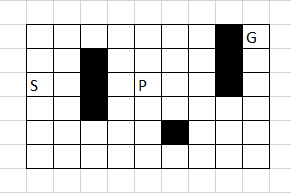
\includegraphics[scale=0.5]{img/simpleMaze.png}
\caption{Sutton's Dyna maze \label{simpleMaze}}
\end{figure}

In order to compare our results with those of \cite{wiering2008}, we used
the same learning rates, discount factors and greediness (inverse of
Boltzmann temperature) parameters. In their paper, they explain how they
tested a wide range of parameters to optimize each of the five RL
algorithms final performance (by evaluating the average reward). They
wanted to compare the best version of each algorithm, which was not
possible if the same parameters were used. For the ensemble methods,
they used the same parameters as were determined for the single RL
algorithms. \cite{wiering2008} observed the discount factor to have a major
impact on the final and cumulative score. For the SARSA method, discount
factors 0.90 and 0.95, and for the ACLA method, discount factors 0.99
and 0.90 were compared to each other. We wanted to confirm these
findings, so we did simulations with the same discount factors.


\begin{table*}
\centering
\begin{tabular}{|l|llllll|}
\hline
Method & \(\alpha\) & \(\beta\) & \(\gamma\) & G & Final &
Cumulative \\ \hline
Q & 0.2 & - & 0.9 & 1 & 5.20 +/- 0.19 & 89.66 +/- 4.82\\
SARSA & 0.2 & - & 0.9 & 1 & 5.20 +/- 0.18 & 91.08 +/-
4.16\\
AC & 0.1 & 0.2 & 0.95 & 1 & 5.21 +/- 0.20 & 95.12 +/-
5.96\\
QV & 0.2 & 0.2 & 0.9 & 1 & 5.21 +/- 0.18 & 92.24 +/- 4.08\\
ACLA & 0.005 & 0.1 & 0.99 & 9 & 5.18 +/- 0.14 & 85.32 +/-
3.59\\
Majority Voting & - & - & - & 1.6 & 5.19 +/- 0.19 & 94.46 +/-
3.63\\
Rank Voting & - & - & - & 0.6 & 4.89 +/- 0.29 & 88.80 +/-
6.74\\
Boltzmann Mult. & - & - & - & 0.2 & 5.23 +/- 0.15 & 94.00 +/-
2.99\\
Boltzmann Add. & - & - & - & 1 & 5.04 +/- 0.32 & 93.18 +/-
6.97\\ \hline
\end{tabular}
\end{table*}

\begin{table*}
\centering
\begin{tabular}{|l|llllll|}
\hline
Method & \(\alpha\) & \(\beta\) & \(\gamma\) & G & Final &
Cumulative  \\ \hline
SARSA & 0.2 & - & 0.95 & 1 & 4.96 +/- 0.90 & 87.04 +/-
17.08\\
ACLA & 0.005 & 0.1 & 0.9 & 9 & 4.27 +/- 1.8 & 60.87 +/-
29.48\\ \hline
\end{tabular}
\end{table*}

\subsubsection{Neural networks as universal function
approximators}\label{neural-networks-as-universal-function-approximators}

Traditionally RL algorithms use tabular expression to represent a
state-function or action-function. In Q-learning for example, a Q-value
is remembered for each state-action combination. Each time the agent
performs an action, gains experience, the Q-value of that specific
state-action pair is updated. For complex games however, there is an
explosion of state-action possibilities. Therefore function
approximators are used to approximate such state(-action) functions,
which try to capture the essence, most essential concepts in order to
maximize reward. Neural networks are universal function approximators,
this mean that a neural network with a single hidden layer containing a
finite number of neurons can approximate any mathematical function to
any desired accuracy. For the more complex mazes of experiments 2 to 5,
we implemented a neural network that was trained after each move of the
agent. Weights were updated after each move using gradient descent for
one iteration. This was done by performing one forward and one backward
propagation pass.

\subsubsection{Partially observable
maze}\label{partially-observable-maze}

For the partially observable maze experiment, we started from the same
Sutton's Dyna maze. However in this case, the starting position varies
and is unknown to the agent. Additionally, the agent can only observe
part of the maze. After each action, it receives an observation, a tuple
of four values (representing the tiles North, South, East and West of
the agent). for example, if there is a wall to the North, a border to
the East and empty tiles in the other directions, the observation tuple
looks like (1,0,1,0). In addition to the 20 \% noise of action
selection, there is also a 10 \% observational noise for each
independent tile. Because the position is unknown to the agent, Markov
localization is used to keep track of a believe state. Initially this
believe state has a uniform distribution over all the tiles without
obstacle. Updates are performed as following:

\[ b_{t+1}(s) = \eta P(o_{t+1}|s) \sum_{s'}T(s',a_t,s) b_t(s') \]

\(a_t:\) action at time t

\(b_t(s):\) believe state

\(o_{t+1}:\) observation

\(\eta:\) normalization factor

\(T(s',a_t,s):\) transition function that maps the state-action pairs to
a probability function over successor states.

Since there are to many states for tabular expression, a neural network
with 20 sigmoidal hidden neurons was used as function approximator. As
input, the network received the believe state as input, a tuple of
length 54.

\subsubsection{Maze with dynamic
obstacles}\label{maze-with-dynamic-obstacles}

For third experiment, 4 to 8 obstacles (walls) were generated at random
locations at the start of each trial. Start and goal positions were
fixed in the same place as Sutton's Dyna maze. If no possible path
exists from start to goal, the agent would not have to solve it and an
new maze was generated instead. The agent needed to learn the knowledge
of a path planner. For this a neural network was implemented with 60
sigmoidal hidden units. As input, the network received a tuple of length
108 (since there are 54 tiles in the maze and we want to know from each
tile whether an agent or wall is on it). 54 of them depict the agent
position (0 or 1 for each tile), and 54 depict the wall positions (0 or
1 for each tile).

\subsubsection{Maze dynamic goal
positions}\label{maze-dynamic-goal-positions}

The fourth maze is very similar to the third maze. Instead of dynamic
obstacles, there is a dynamic goal position. Obstacles and starting
position are placed as in Sutton's Dyna maze. This time, a neural
network with 20 sigmoidal hidden units and a tuple of length 108 as
input was used as function approximator. This time 54 values represent
the agent position, and the other 54 values the goal position.

\subsubsection{Generalized maze}\label{generalized-maze}

The last experiment combined the problem of a maze with dynamic
obstacles and a maze with dynamic goals positions into a generalized
maze experiment (wierling 2008 {[}23{]}). In this maze, the goal and
obstacles are positioned at random positions at the start each trial. A
neural network with 100 sigmoidal hidden units receives 162 (54x3) input
values, 54 to describe the agent position, 54 to describe the obstacle
positions, and 54 to describe the goal position.

\begin{figure*}
\centering
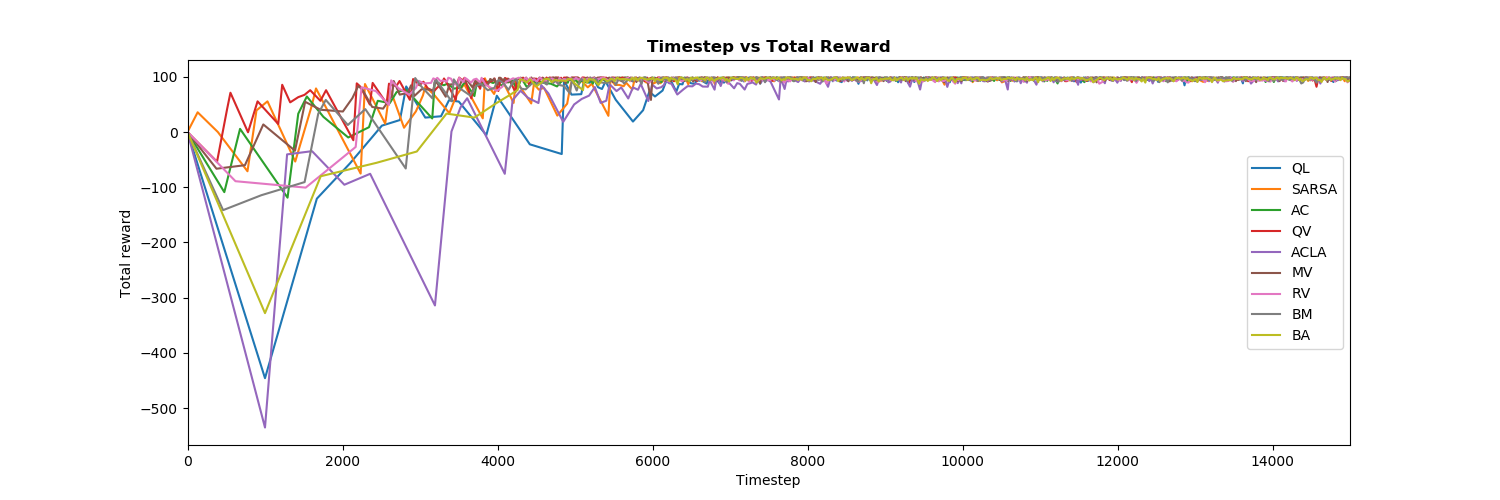
\includegraphics[scale=0.35]{img/Timestep_vs_Total_reward_simple.png}
\caption{Figure 2}
\end{figure*}

\begin{figure*}
\centering
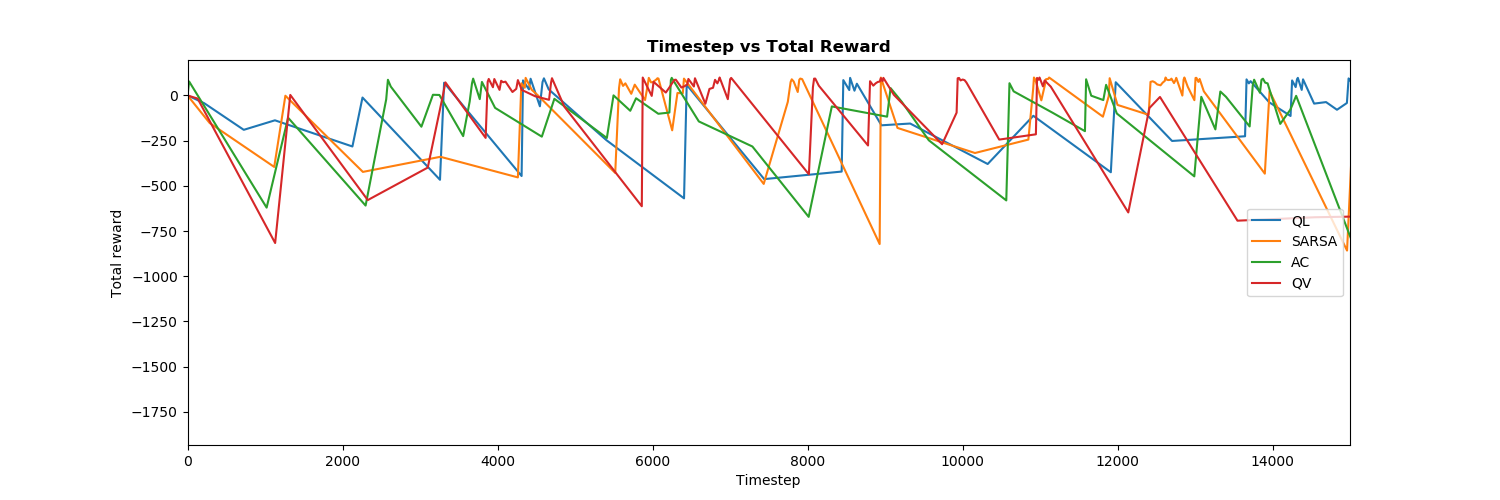
\includegraphics[scale=0.35]{img/Timestep_vs_Total_reward.png}
\caption{Figure 3}
\end{figure*}

\section{Results}\label{results}
\subsection{Simple Maze}\label{simple-maze}

The evaluation was done by noting the Final Reward intake during the
last 2500 learning-steps of each simulation. Also the cumulative average
reward was calculated after every 2500 learning-steps. Each simulation
has 50,000 learning-steps. Table 1 shows the average results and the
standard deviation of 500 such simulations.

It was observed that Majority voting and Boltzmann Multiplication have
the best Final as well as the Cumulative reward intakes. In the current
experiment, Boltzmann addition has the worst performance.

In order to examine the effect of the discount factor (\(\gamma\)) , the
SARSA and the ACLA algorithms are rerun with different discount factors.
The results are shown in table 2.

 There is a significant drop in the performance of both algorithms as
compared to the previous simulations.

Figure 1 and 2 plots the total reward obtained by the algorithms vs the
timestep. For the sake of clarity results are plotted till 15,000
timesteps. It can be observed that all algorithms converge to a stable
performance well within 15,000.

\subsection{Maze with dynamic
obstacles}\label{maze-with-dynamic-obstacles-1}

Figure 3 plots the total reward over time steps for a Maze with Dynamic
obstacles. None of the algorithms successfully converge to stable
values. Consequently the final and the cumulative rewards are negative,
which is far below that of simple maze.

\section{Discussion}\label{discussion}

Although the article of \cite{wiering2008} is very interesting and shows new
insights, we are of the opinion that they could have taken extra steps
to assure reproducibility. Some methods were ambiguously explained, so
that it took some effort to figure out what was meant exactly. The
source was also not available, which would have solved previous remark.
For example, while implementing the neural network, it is not clear how
the weights are updates. We decided to update the weights after each
move gradient descent for one iteration. However, it is possible that in
the original paper, they used multiple gradient descent iterations after
each move. Or maybe, action replay as in, ``Human-level control through
deep reinforcement learning'', from DeepMind where used. Here, actions,
states and rewards are stored in memory and every so often, the weights
are updated by learning from the experiences stored in memory. This
could be one of the reason why our neural networks were not able to
converge for the dynamic maze and other more complex maze experiments,
while in the original paper, they did. Other possible explanation are
numerical errors.

For the small maze experiment, we observed very similar results to those
in the paper. All final and cumulative values were within the standard
deviation.

\cite{wiering2008} determined all learning parameters by performing various
trials with different parameter values. They noted in their paper that
the discount factor had a major effect on the performance. To assess
this effect, the SARSA and the ACLA algorithms were trained on the
simple maze with changed discount. We observe a significant change in
the final and the cumulative reward, which highlights the importance of
this parameter in the overall performance of the algorithms.

\footnotesize
\bibliographystyle{apalike}
\bibliography{sources}


\end{document}

